\subsection{Introducci\'on}
En este \'ultimo Trabajo Pr\'actico de la materia vamos a afrontar la resoluci\'on del problema de encontrar una k-Partici\'o de Peso M\'inimo (de ahora en m\'as k-PMP), el cual se trata de un problema que pertenece a la clase NP-Completo\footnote{http://en.wikipedia.org/wiki/Minimum\_k-cut} y por lo tanto no se conoce un algoritmo en tiempo polinomial que lo resuelva.\\
Por tal motivo, vamos a buscar una soluci\'on exacta mediante un BackTraking y luego realizar algoritmos aplicando distintas heur\'isticas (Golosa, Busqueda Local, GRASP) para analizar las ventajas y desventajas de cada una.

\subsection{Problema}

Dado un grafo simple $G = (V, E)$ y un entero $k$, se define una k-partici\'on de G como una partici\'on de V en k conjuntos de v\'ertices $V_{1} , \ldots , V_{k}$. Las aristas intrapartici\'on de una k-partici\'on, son aquellas aristas de G cuyos extremos se encuentran en un mismo conjunto de la partici\'on, es decir, una arista $uv \in E$ es intrapartici\'on si existe un $i \in {1, \ldots , k}$, tal que $u, v \in V_{i}$ . Dada una función de peso $\omega : E \rightarrow \mathbb{R}_+$, definida sobre las aristas de G, el peso de una k-partici\'on es la suma de los pesos de las aristas intrapartici\'on.

El problema $k$-PMP consiste en encontrar, dado un grafo simple $G = (V, E)$, un entero $k$ y una función $\omega : E \rightarrow \mathbb{R}_+$, una $k$-partición, que tenga a lo sumo $k$ subconjuntos, de $V$ con peso mínimo.

\subsection{Ejemplos}
En el seiguiente ejemplo vamos a ver lo que ser\'ia una partici\'on cualquiera del grafo y luego la k-PMP

Se el siguiente grafo: 

\bc
		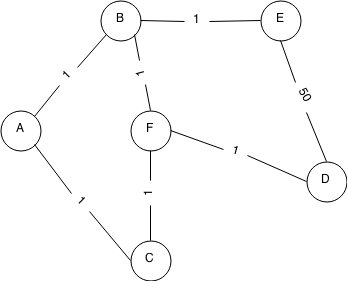
\includegraphics[scale=0.5]{img/kpmp.png}
\ec

Podemos realizar la siguiente 2-partici\'on 

\bc
		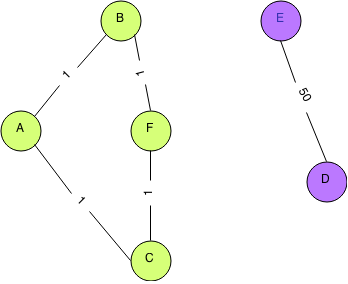
\includegraphics[scale=0.5]{img/kpmp1.png}
\ec

Se puede apreciar f\'acilmente que esta partici\'on no cumple que sea m\'inima dentro de todas las 2-particiones posibles. Pues el peso total es de 54. Y por ejemplo existe la siguiente 2-particion en donde la suma del peso de sus aristas intraparticiones es igual a 0.

\bc
		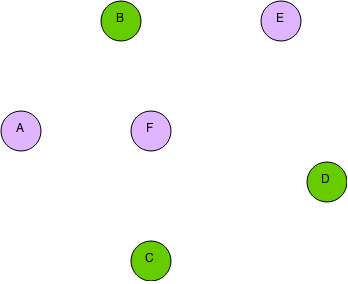
\includegraphics[scale=0.5]{img/kpmp2.png}
\ec